

\chapter{Results and Discussion}

\section{Numerical Verification of Advection}

The first task involved testing the Upwind finite difference scheme using a $2D$ advection problem. The numerical results for the velocity components $v$ and $w$ were compared against the analytical solutions. For a $100 \times 100$ grid, we observed a maximum error of approximately $0.38$ for $v$ and $0.42$ for $w$ (See Figure \ref{fig:Introduction}). This level of error is consistent with first-order numerical schemes, which are known for introducing numerical diffusion, causing the profiles to dampen over time.
This dampening can be seen in figure \ref{fig:Introduction}: 
Local extrema are slightly less pronounced in the numerical solutions (indicated by slightly weaker blue and yellow intensity). 
Additionally, the transition from extrema to non-extreme locations is 'smoother' in the numerical solutions.
Vice versa, we can observe sharper color transitions in the analytical solution.
Although this phenomenon is difficult to spot optically, it indicates the numerical diffusion property.
\begin{figure}[H]
    
    \centering
    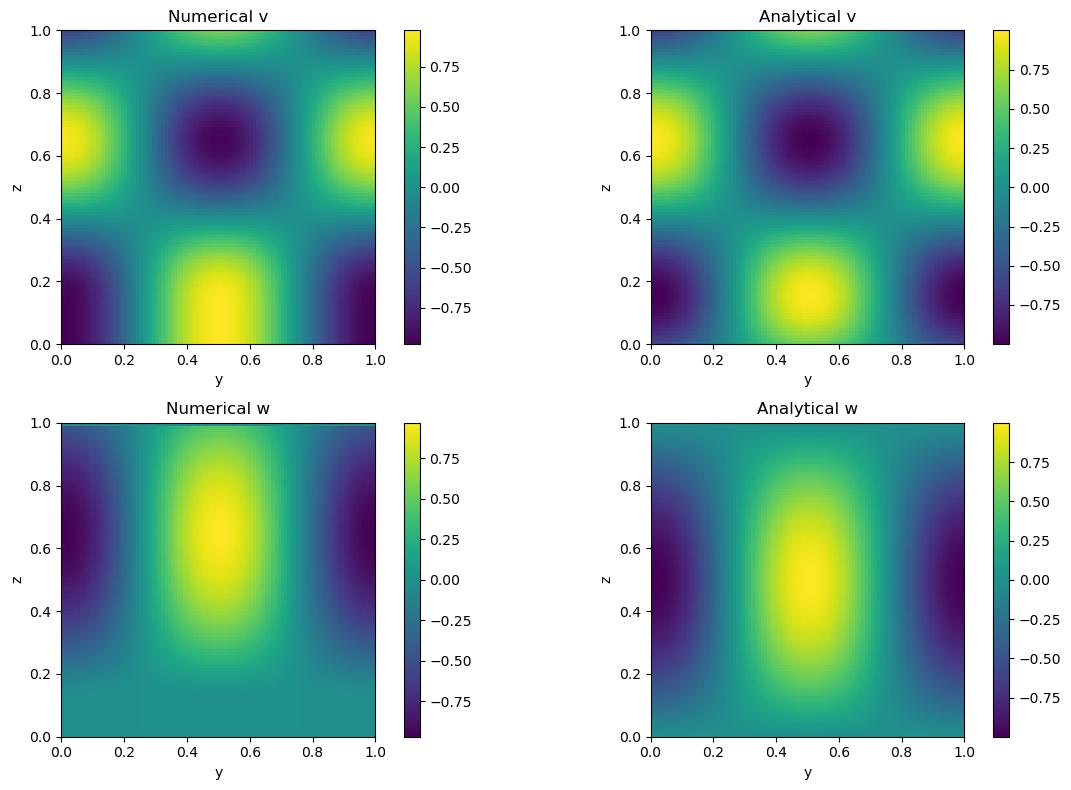
\includegraphics[width=0.9\textwidth]{Images/velocity.jpeg}
    \caption[Comparison of analytical and numerical results]{Comparison of analytical and numerical solutions in advection test.}
    \label{fig:Introduction}
\end{figure}

Concluding, the implementation of a numerical solver for the linear advection was successful.
We used operator splitting to enhance computational efficiency and respected the given boundary conditions.
In the next subtask, we had to extend the simple linear advection case by the incompressibility constraint.

\section{Analysis of the Projection Method Step}
\subsection{Stability and Time-Stepping}

The use of an Explicit Euler scheme necessitates a strict adherence to the Courant (CFL) condition. In our simulations, a time step of the order of magnitude of $\Delta t \approx 10^{-3}$ was chosen to maintain a Courant number below ${1}$. Although an implicit scheme would allow for larger time steps, the current explicit implementation provides a clear and computationally straightforward approach to studying transient Rayleigh-Benard convection cells without the excessive computational costs of massive matrix inversions.

We considered two options for the numerical approach: Explicit Euler and Implicit Euler. If we chose Explicit, we had to tune the solver with many simple, ``cheap'' time steps governed by strict stability limits ($CFL < 1$). If we opted for the Implicit approach, we would have executed fewer, ``expensive'' time steps that are stable at larger intervals but require heavy matrix calculations. Eventually, due to fewer complexities and need for stronger processors, we employed the Explicit Euler method for our numerical approach.

We were surprised that such 'simple' methods modelled the flow accurately.


\begin{table}[H]
    
    \centering
    
    \begin{tabular}{llll}
        \toprule
        \textbf{Solver Type} & \textbf{Iterations / Method} & \textbf{Max Div.} & \textbf{Status Analysis} \\
        \midrule
        Initial Jacobi      & 1,000 Iterations & $1.894$                   & Unstable / Unacceptable \\
        Optimized Jacobi    & 5,000 Iterations & $5.55 \times 10^{-2}$     & Moderate Accuracy (5\% error) \\
        FFT (Final Version) & Direct Solver    & $\approx 10^{{-6\:to \:-16}}$    & Ideal (Machine Precision) \\
        \bottomrule
    \end{tabular}
    \caption[Divergence Comparison]{\textbf{Divergence Comparison.} Divergence analysis for the numerical solution of the Poisson equation for different numerical methods. The maximum value of divergence as a measure for the successful implementation of the incompressibility can be found in the third column from the left.}
    \label{tab:divcomparison}
\end{table}
The implementation of the incompressibility lead to a Poisson equation which constrained the pressure of our simulation.
Thus, the pressure field is calculated after we ensured $\nabla \textbf{u} = 0$ (incompressibility condition) and should be near zero for a physically correct simulation.
The correction of the pressure values led to a computational challenge and turned out to be crucial for the convergence of our numerical procedure.
To reduce the divergence in the velocity field we applied different Poisson solver.
 
%\subsection{Incompressible Flow Performance}

The core of the simulation, the Chorin's projection method, was tested for mass conservation (see table \ref{tab:divcomparison}). In the initial implementation, the maximum divergence of the velocity field was high ($1.8$, see table \ref{tab:divcomparison}), indicating poor pressure correction. After refining the Neumann boundary conditions for the pressure Poisson solver and ensuring the grid spacing correctly accounts for the wall boundaries, the maximum divergence was significantly reduced to $5.55 \times 10^{-2}$. This confirms that the projection step is effectively enforcing the incompressibility constraint $\nabla \cdot \mathbf{u} \approx 0$.

Since the Jacobi method has a slow convergence rate for high-frequency errors, increasing the number of iterations or employing a more robust solver like the Conjugate Gradient method (CG) or Fast Fourier Transform (FFT) would further drive the divergence towards machine epsilon.
This reduction of divergence by using Fast-Fourier-Transformation is further elaborated in section \ref{sec:poisson solver}.


\begin{figure}[H]
    \centering
    \begin{subfigure}{1.0\textwidth}
        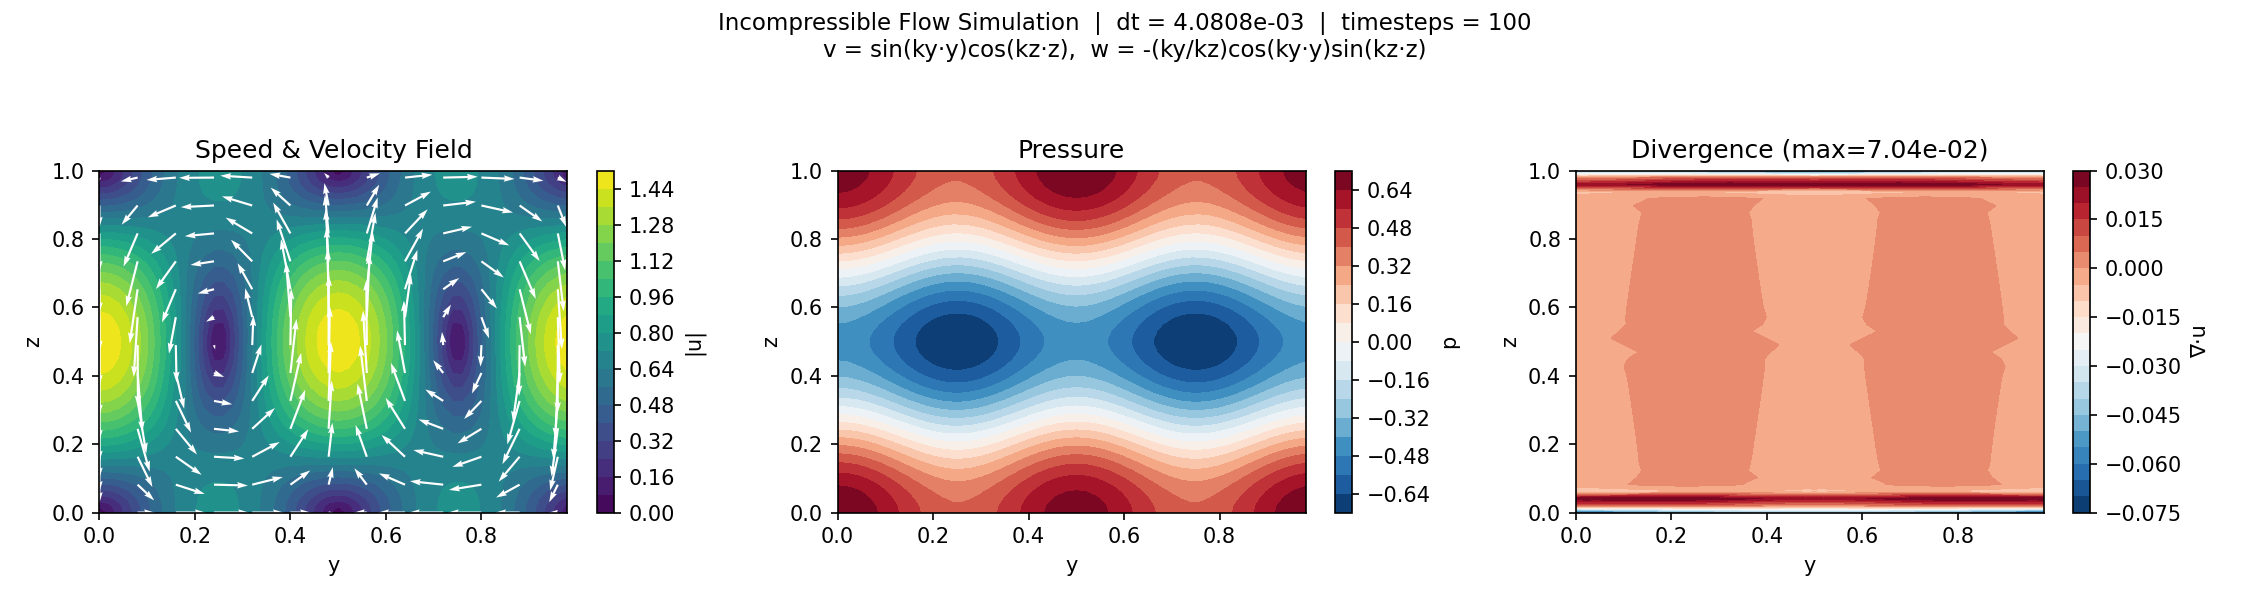
\includegraphics[width=\textwidth]{Images/incompressible_flow__mode1.png}
    \end{subfigure}
    \begin{subfigure}{1.0\textwidth}
        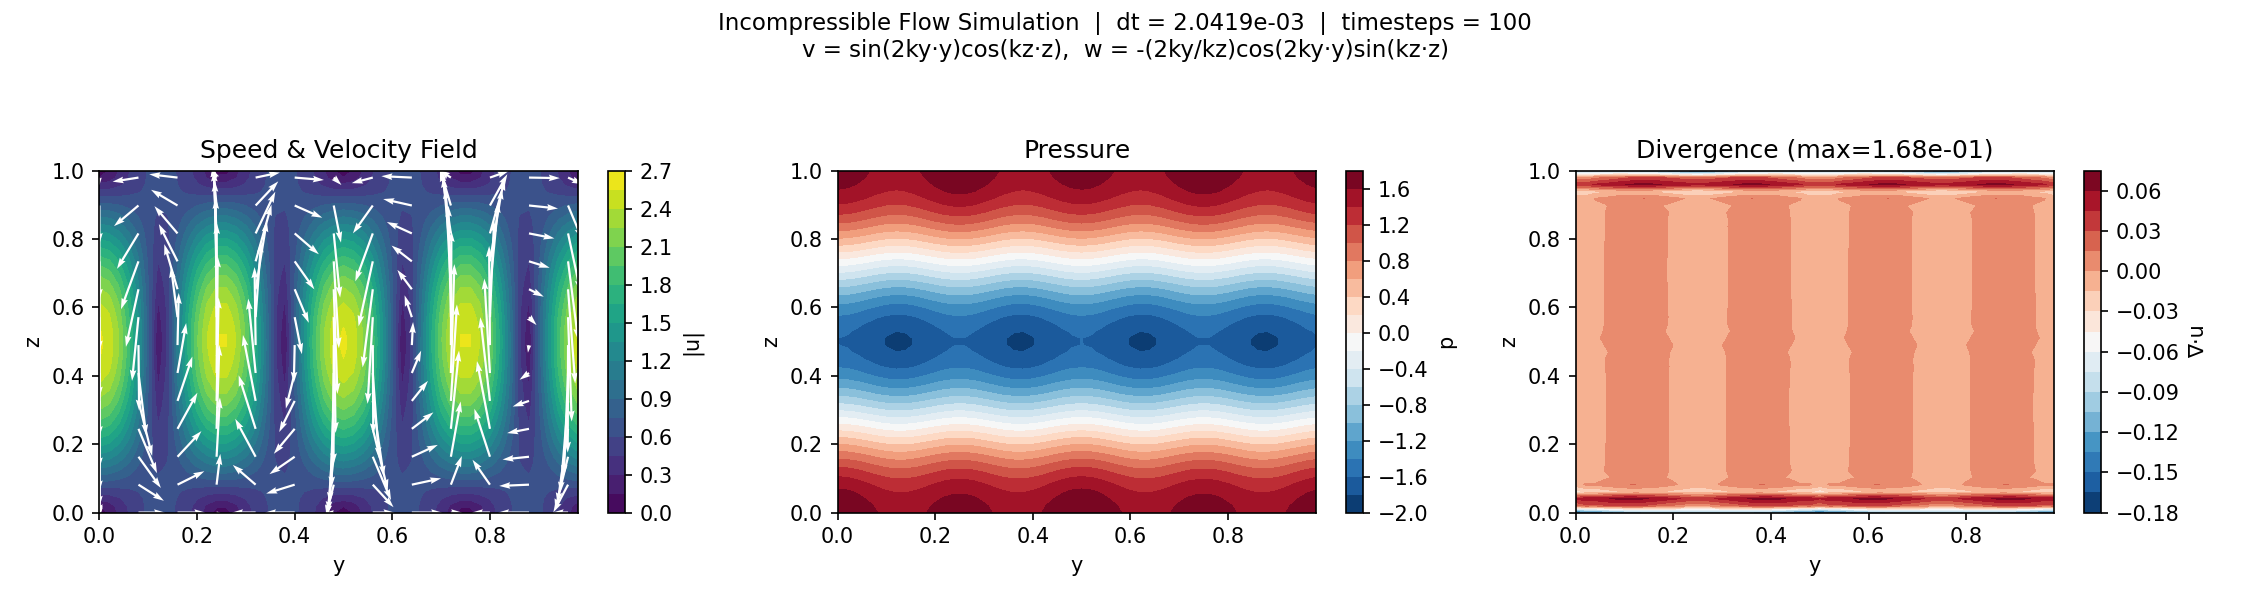
\includegraphics[width=\textwidth]{Images/incompressible_flow__mode2.png}
    \end{subfigure}
    \begin{subfigure}{1.0\textwidth}
        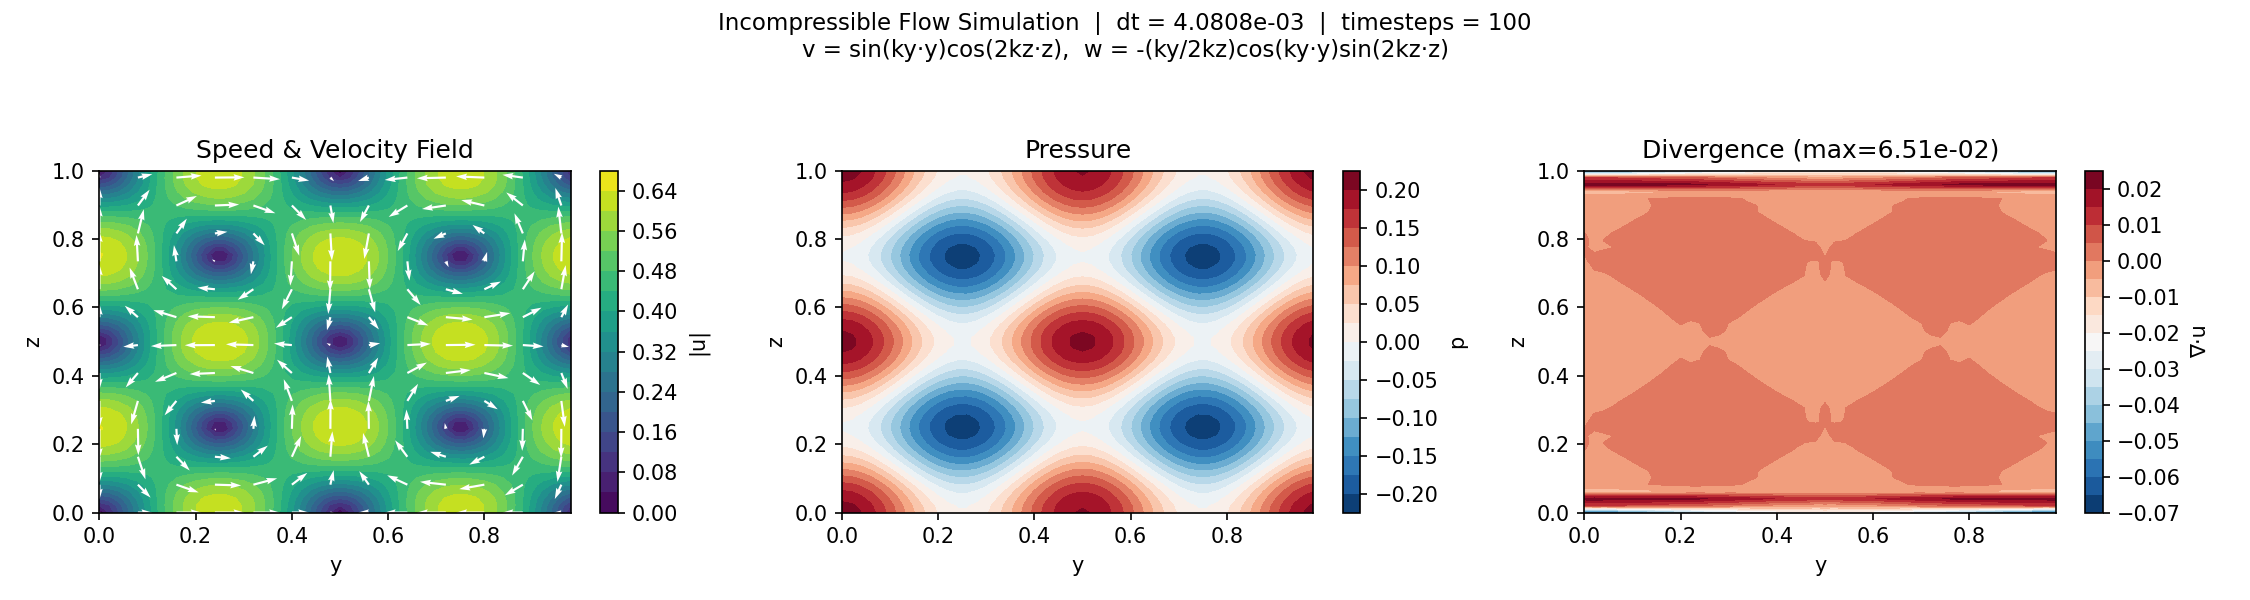
\includegraphics[width=\textwidth]{Images/incompressible_flow__mode3.png}
    \end{subfigure}
    \begin{subfigure}{1.0\textwidth}
        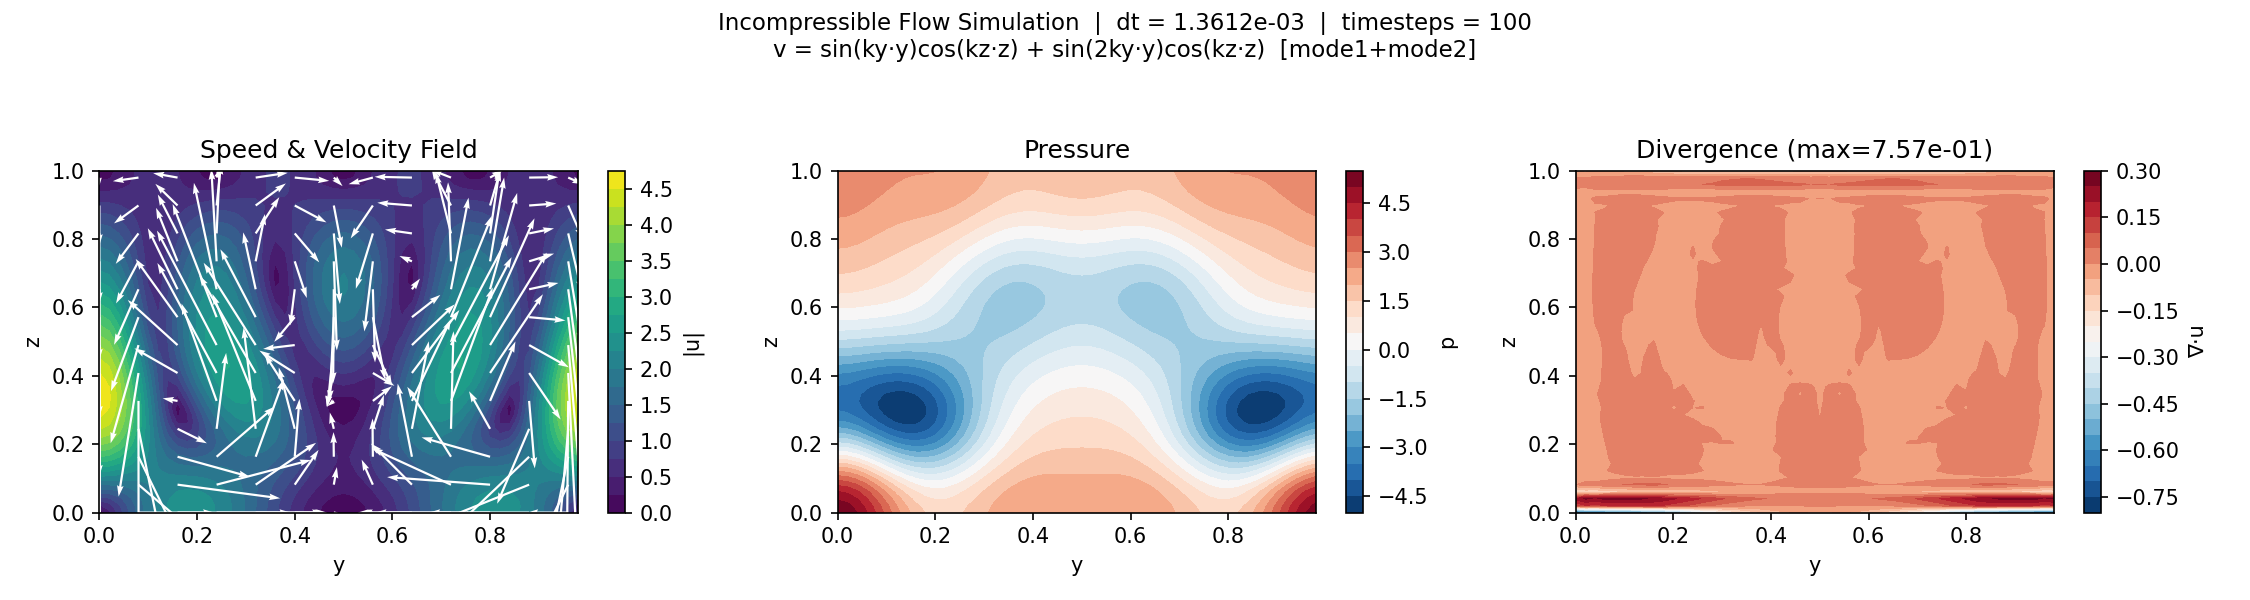
\includegraphics[width=\textwidth]{Images/incompressible_flow__double.png}
    \end{subfigure}
    \caption[Simulated flow]{\textbf{Resulting simulation results.} Flow behavior for different parameterisations. Numerical calculations have been performed by using FFT and spectral decomposition.}
    \label{fig:dtcomparison}
\end{figure}


In figure \ref{fig:dtcomparison} we can see, that the implementation of spectral methods to tackle the solution of the Poisson equation is successful.
Different modes lead to different spatial distributions of pressure and divergence.
But for all simulations we obtain bounded values in divergence implying convergence of the numerical method.
In the last row, the superposition of the different modes is showing increased complexity in flow behaviour.
We therefore consider the use of spectral methods (such as FFT and DCT) as successful.

Additionally, computational cost could be reduced and we expect increased accuracy for enhanced spatial and temporal resolution.
Intuitively, the reduction in computational cost would easily allow such an increased resolution.
But for our simulation we did not systematically compare different resolutions as simulation results were already satisfying physical behaviour.
Nevertheless, for the last part, the use of FFT and spectral methods regarding the Poisson equation were especially important to produce realistic convective behavior.


\section{Rayleigh-Benard Convection}

\subsection{Poisson Solvers: Divergence analysis}\label{sec:poisson solver}
In the previous sections, forcing was ignored when the Navier-Stokes equations were solved.
But for the last task, the model was further extended by incorporating the temperature ($T$) advection-diffusion equation and coupling it with the Navier-Stokes equations. The buoyancy term, scaled by coefficient $\beta$, was added to the vertical velocity ($w$) equation to simulate the thermal effects on fluid motion, which would be rising of warm air and sinking of cold air.
As we still had to respect the incompressibility constraints, the solution of the Poisson equation by Chorin's Projection method remained a central numerical challenge.
We explored two distinct approaches

\subsection*{Jacobi Iterative Method}

The resulting divergence of the Jacobi method exhibited values of up to $0.055$. 
These values were too high to reproduce the successful reproduction of convection cells.
Unrealistic behavior occurred and can be observed in figure \ref{fig:divjacobi}.
We see that the spatial distribution of high values of divergence is inhomogeneous.
Around the top ($z=1.0$) and bottom ($z=0.0$) of our simulated domain, the divergence values are peak.
As we were in need of further reducing the divergence as a result of unrealistic simulation output, we tested spectral methods for the solution of the Poission equation.

\begin{figure}[H]
    \centering
    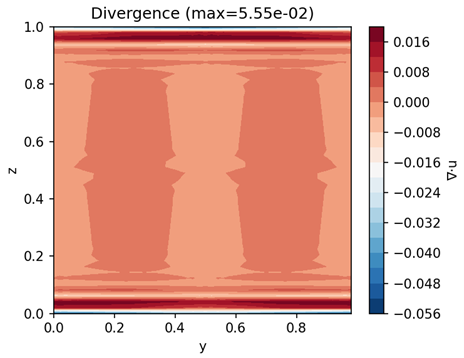
\includegraphics[width=0.5\textwidth]{Images/JacobiDivergence.png}
    \caption[Divergence Jacobi method]{Divergence field in the Jacobi method. Max Divergence $= 5.55 \times 10^{-2}$.}
    \label{fig:divjacobi}
\end{figure}


\subsection*{Fast Fourier Transform (FFT) Method}

In the final version of our implementation, the Poisson solver was replaced by an FFT-based approach. This method transforms the problem from the spatial domain to the frequency domain, where complex derivatives become simple algebraic divisions.


\begin{figure}[H]
    \centering
     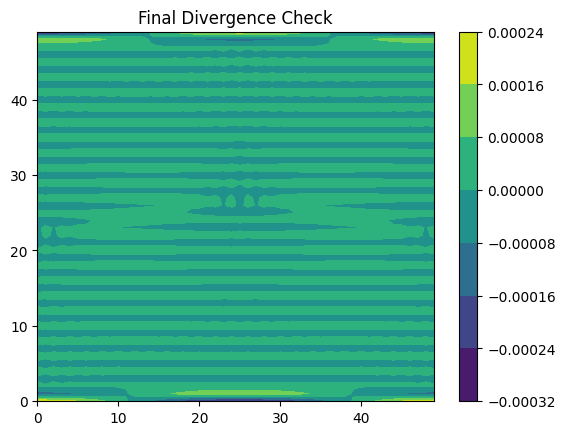
\includegraphics[width=0.6\textwidth]{Images/FinalDivergenceCheck.png}
    \caption[Divergence FFT]{Divergence error at machine precision accuracy using FFT solver.}
    \label{fig:divfft}
\end{figure}

The primary challenge in previous versions of numerical solutions was the high divergence caused by the limitations of the Jacobi iterative solver in handling the Poisson equation. By replacing it with the Fast Fourier Transform (FFT) method, the maximum divergence was reduced from $10^{-2}$ to approximately $10^{-15}$. A spatial distribution of the divergence values is given in figure \ref{fig:divfft}. We can clearly observe uniform low values for this method across the entire domain. 
This transition not only achieved machine-precision accuracy but also significantly accelerated computational performance.
Reaching divergence $\approx 10^{-6}$  signifies that the principle of mass conservation is almost perfectly satisfied. This resolves a major bottleneck in the CFD code, providing a robust foundation for the thermal simulation.


\section{Rayleigh-B\'{e}nard Convection Results}
The last task consisted of finding suitable initial conditions and parameterization that would lead to convective behaviour.

\begin{figure}[H]
    %\centering
    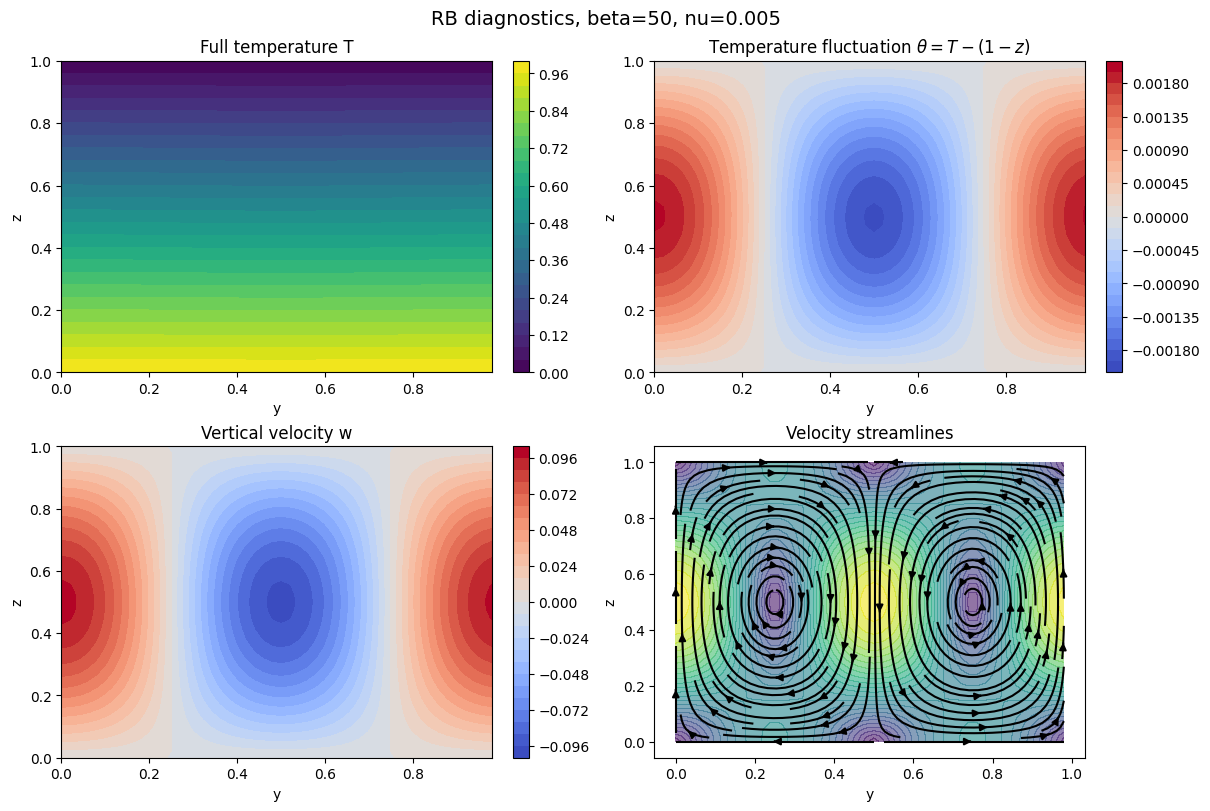
\includegraphics[width=1.05\textwidth]{Images/RB_Diagnostics.png}
    \caption[Rayleigh-B\'{e}nard convection cells]{\textbf{Results of the numerical solution for $\beta = 50,\: \nu = 0.005$.} Results for a paramterisation causing Rayleigh-B\'{e}nard convection cells induced by thermal forcing (for thermal forcing see plot at the upper left).}
    \label{fig:convecresults}
\end{figure}

The simulation efficiently exhibits the formation of classical convection cells for the implementation of all previously described numerical methods, with the buoyancy term $\beta =50.0$ and viscosity $\nu =0.005$. 
The results in Figure \ref{fig:convecresults} illustrate the formation of Rayleigh-Benard convection. The temperature fluctuation figure shows the temperature deviation from the conductive profile in the previous stage. It displays alternating warm and cold regions, such that warm fluid rises from the heated bottom, while cooler fluid -when reaches the top- sinks from there. In the Vertical velocity field w, the motion appeared due to the temperature difference. This result confirms the motion caused by convective heat transfer. The Regions of higher temperature, warm plumes in red, correspond to upward flow, and colder regions, cold plumes in blue, correspond to downward motion. In the final part of this figure, the flow field streamlines can be observed, displaying two counter-rotating convection rolls. The streamlines clearly show that the hot fluid rises from the bottom, spreads horizontally near the top, cools there, and then descends along the sides. This circulation pattern is the characteristic of the two-D Rayleigh-Benard convection cells.
These circulation patterns confirm the simulation's success in capturing Rayleigh-B\'{e}nard physics and the stability of the numerical method under periodic (in $y$) and wall-bounded (in $z$) boundary conditions.